\documentclass[12pt,a4paper]{article}
\usepackage{cmap} % Makes the PDF copiable. See http://tex.stackexchange.com/a/64198/25761
\usepackage[T1]{fontenc}
\usepackage[brazil]{babel}
\usepackage[utf8]{inputenc}
\usepackage{amsmath}
\usepackage{amsfonts}
\usepackage{amssymb}
\usepackage{amsthm}
\usepackage{textcomp} % \degree
\usepackage{gensymb} % \degree
\usepackage[usenames,svgnames,dvipsnames]{xcolor}
\usepackage{hyperref}
\usepackage{multicol}
\usepackage{graphicx}
\usepackage[margin=2cm]{geometry}
\usepackage{icomma} % vírgulas como pontuação vs ponto decimal
\hypersetup{
    colorlinks = true,
    allcolors = {blue}
}

\newcommand{\fixme}{{\color{red}(...)}}
\newcommand*\sen{\operatorname{sen}}
\newcommand*\tg{\operatorname{tg}}
\newcommand*\arctg{\operatorname{arctg}}
\newcommand*\R{\mathbb{R}}
\newcommand*\diff{\mathop{}\!\mathrm{d}}

\newcommand{\IconPc}{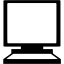
\includegraphics[width=1em]{computer.png}}
\newcommand{\IconCalc}{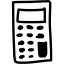
\includegraphics[width=1em]{calculator.png}}
\newcommand{\IconThink}{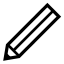
\includegraphics[width=1em]{pencil.png}}
\newcommand{\IconCheck}{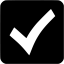
\includegraphics[width=1em]{checkmark.png}}
\newcommand{\IconConcept}{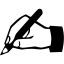
\includegraphics[width=1em]{edit.png}}

\newlength{\SmileysLength}
\setlength{\SmileysLength}{\labelwidth}\addtolength{\SmileysLength}{\labelsep}

\newcommand{\calc}{\hspace*{-\SmileysLength}\makebox[0pt][r]{\IconCalc}%
   \hspace*{\SmileysLength}}
\newcommand{\software}{\hspace*{-\SmileysLength}\makebox[0pt][r]{\IconPc}%
   \hspace*{\SmileysLength}}
\newcommand{\teoria}{\hspace*{-\SmileysLength}\makebox[0pt][r]{\IconThink}%
   \hspace*{\SmileysLength}}
\newcommand{\conceito}{\hspace*{-\SmileysLength}\makebox[0pt][r]{\IconCheck}%
   \hspace*{\SmileysLength}}
\newcommand{\concept}{\hspace*{-\SmileysLength}\makebox[0pt][r]{\IconCheck}%
   \hspace*{\SmileysLength}}

\newcommand*\tipo{3ª Lista de Exercícios}
%\newcommand*\turma{...}
\newcommand*\disciplina{ANN0001/CAN0001}
\newcommand*\eu{Helder G. G. de Lima}
\newcommand*\data{\today}

\author{\eu}
\title{\tipo - \disciplina}
\date{\data}

\begin{document}

\begin{center}

\includegraphics[width=9.0cm]{marca} \\
\textbf{\tipo\ (\disciplina)} \\
Prof. \eu\footnote{
Este é um material de acesso livre distribuído sob os termos da licença \href{https://creativecommons.org/licenses/by-sa/4.0/deed.pt_BR}{Creative Commons BY-SA 4.0}.}
\end{center}

%\section*{Legenda}
%\begin{multicols}{4}
%\begin{itemize}
%\item[] \hspace*{\SmileysLength} \calc \hspace*{-\SmileysLength} Cálculos
%\item[] \hspace*{\SmileysLength} \conceito \hspace*{-\SmileysLength} Conceitos
%\item[] \hspace*{\SmileysLength} \teoria \hspace*{-\SmileysLength} Teoria
%\item[] \hspace*{\SmileysLength} \software \hspace*{-\SmileysLength} Software
%\end{itemize}
%\end{multicols}

\section*{Questões}

\begin{enumerate}
\item Obtenha a reta que melhor se ajusta (por mínimos quadrados) aos pontos
$A = (-3, -5)$,
$B = (-2,  7)$,
$C = (-1,  0)$,
$D = ( 0,  1)$,
$E = ( 1,  2)$,
$F = ( 2,  1)$,
$G = ( 3,  2)$,
$H = ( 4,  1)$.
\item Utilize a regressão por mínimos quadrados para ajustar (a) uma reta, (b) uma parábola e (c) uma função da forma $f(x) = k_1 + k_2 \cos(\pi x) + k_3 x^2$ aos seguintes dados, e determine em qual dos três casos o erro quadrático é menor:
\begin{center}
\begin{tabular}{|c|c|c|c|c|c|c|c|}
\hline
   $x_i$ & -3 & -2 & -1 &  0 & 1 & 2 & 3 \\ \hline
$y_i$ & 14 &  4 &  4 & -2 & 2 & 0 & 8 \\
\hline
\end{tabular}
\end{center}

\item Considere um conjunto de pontos $D = \{(x_1,y_1), \ldots, (x_n,y_n)\}$. Classifique as afirmações a seguir como verdadeiras ou falsas, justificando suas respostas:
\begin{enumerate}
\item A função afim que melhor se ajusta a $D$ nunca tem o mesmo erro/resíduo quadrático que o polinômio de grau no máximo dois que melhor se ajusta a $D$.
\item O resíduo quadrático de uma função $f(x) = a_1 + a_2 x$ que melhor se ajusta a $D$ sempre é maior ou igual ao de uma função $g(x) = a_1 + a_2 x + a_3 x^2$ que melhor se ajusta a $D$.
\item O resíduo quadrático da reta que melhor se ajusta a $n$ pontos é maior ou igual ao da reta que se ajusta a $n-1$ destes mesmos pontos.
\end{enumerate}

\item Obtenha a função racional do tipo $f(x) = \frac{a}{x} + \frac{b}{x^2}$ que melhor se ajusta aos pontos do conjunto $D = \{ (1, 3), (2, 0), (2, -2), (5, -1) \}$, no sentido dos mínimos quadrados.

\item Seja $D = \{ (-1,2), (0,3), (1, k) \}$. Determine os valores de $k \in \R$ para os quais o erro quadrático da reta que melhor se ajusta a $D$ é menor do que $2/3$.

\item Encontre as funções afins que melhor se ajustam, no sentido dos mínimos quadrados a:
\begin{multicols}{2}
\begin{enumerate}
   \item $f(x) = e^x$ no intervalo $[-1, 1]$.
   \item $f(x) = \cos(x)$ no intervalo $[0, \pi]$.
\end{enumerate}
\end{multicols}

\item Utilize as raízes do polinômio de Chebyshev de grau dois, e (se necessário) uma transformação dos intervalos, para construir um polinômio interpolador de grau menor ou igual a um para as seguintes funções nos intervalos indicados:
\begin{multicols}{2}
\begin{enumerate}
   \item $f(x) = 2^x$ no intervalo $[-1, 1]$.
   \item $f(x) = 2^x$ no intervalo $[0, 3]$.
\end{enumerate}
\end{multicols}

\item Repita o exercício anterior com as raízes do polinômio de Chebyshev de grau três, para obter um polinômio interpolador de grau menor ou igual a dois.

\item Uma forma simples de estimar o valor de $\int_a^b f(x)\diff{x}$ é utilizar o \textit{método do ponto médio}, um método de Newton-Cotes aberto, no qual considera-se um retângulo cuja base é o intervalo $[a,b]$ e a altura é o valor de $f$ no ponto médio deste intervalo, ou seja:
\[
\int_a^b f(x)\diff{x} \approx (b-a) \cdot f\left(m \right),
\quad
m = \frac{a+b}{2}.
\]

Calcule numericamente as integrais a seguir por meio de uma única aplicação das regras: (1) do ponto médio, (2) do trapézio, (3) 1/3 de Simpson, (4) 3/8 de Simpson e (5) de Boole. Obtenha também as soluções exatas e compare-as com as aproximações obtidas, calculando os erros relativos percentuais. Interprete geometricamente.
\begin{multicols}{4}
\begin{enumerate}
\item $\int_0^1 3x^2 \diff{x}$
% I = 1
\item $\int_0^1 4x^3 \diff{x}$
% I = 1
\item $\int_{0}^1 x^9 - 3x^2 \diff{x}$
% I = -0.9
\item $\int_{1}^5 \frac{4}{x} - \cos(x) \diff{x}$
% I ≈ 8.2381
\end{enumerate}
\end{multicols}

\item Considere a integral $I = \int_0^2 \cos(x^2)\diff{x}$, cujo valor com 10 casas decimais corretas é $0.4614614624$. Subdivida o intervalo $[a, b] = [0, 2]$ utilizando $n+1$ pontos igualmente espaçados, $a = x_0 < x_1 < \ldots < x_n = b$, e calcule numericamente o valor aproximado de $I$ aplicando repetidas vezes os métodos do ponto médio, do trapézio e 1/3 de Simpson aos subintervalos $[x_i,x_{i+1}]$. Compare os resultados obtidos com $n = 1, 2, 4, 8$.

\item Seja $M$ a aproximação de $\int_a^b f(x)\diff{x}$ fornecida pela regra do ponto médio, $T$ a aproximação obtida pela regra do trapézio e $S$ a aproximação que resulta da regra 1/3 de Simpson. Mostre que $S$ é uma média aritmética ponderada de $M$ e $T$.

\item Qual é o maior valor de $h \in \mathbb{R}$ para o qual a regra do trapézio aproxima $\int_0^h f(x) \diff{x}$ com um erro absoluto $|\varepsilon_{abs}| \leq 0,1$ considerando que $f(x) = x^2$? E se $f(x) = x^3$, o valor de $h$ aumenta, diminui ou permanece o mesmo? O que se pode esperar de outras funções $f(x) = x^n$, com $n = 4,5,6,\ldots$? Explique.

\item Considere uma função $g$ que assume os valores dados na tabela a seguir:
%g(x) = (x² + 1) cos(x π / 12 )
\begin{center}
\begin{tabular}{|c|c|c|c|c|c|c|c|}
\hline
   $x_i$ & 0 & 1 & 2 & 3 & 4 & 5 & 6 \\ \hline
$g(x_i)$ & 1.00 & 1.93 & 4.33 & 7.07 & 8.50 & 6.73 & 0.00 \\
\hline
\end{tabular}
\end{center}
Estime $\int_0^6 g(x)\diff{x}$ utilizando os métodos a seguir no maior número de subintervalos de mesmo comprimento que for possível:
\begin{multicols}{2}
\begin{enumerate}
\item A regra do trapézio.
\item A regra 1/3 de Simpson.
\end{enumerate}
\end{multicols}

\item Explique uma das regras de integração/quadratura numéricas, e deduza a fórmula correspondente a partir de sua interpretação geométrica.

\item Durante os primeiros segundos após o lançamento de um foguete em direção à lua, foi registrado que sua velocidade aumentava conforme a tabela a seguir:
\begin{center}
\begin{tabular}{|c|c|c|c|c|c|c|c|}
\hline
  $t\ (s)$ & 0 & 10 & 20 & 30 & 40 \\ \hline
$v\ (m/s)$ & 0 & 65,5 & 180,7 & 345,7 & 560,2 \\
\hline
\end{tabular}
\end{center}
Calcule a altura do foguete após 40 segundos utilizando a regra 1/3 de Simpson.

\item Estime as integrais a seguir utilizando a quadratura de Gauss-Legendre com 2 a 5 pontos, depois de realizar uma mudança de variáveis apropriada para usar o intervalo $[-1,1]$:
\begin{multicols}{4}
\begin{enumerate}
\item $\int_0^2 x^2 + x\diff{x}$
\item $\int_1^2 \frac{2}{x^2}\diff{x}$
\item $\int_{-1}^3 e^{-x^2}\diff{x}$
\item $\int_{-3}^3 \frac{1}{1+x^2} \diff{x}$
\end{enumerate}
\end{multicols}

\item Utilize o método de Romberg para estimar o valor de $\pi = \int_{-1}^1 \frac{2}{x^2 + 1}\diff{x}$, com um erro relativo percentual inferior a $0,1\%$.

\item Forneça uma estimativa de $\int_1^{1.8} e^x\diff{x}$ com erro relativo menor ou igual a $10^{-7}$, utilizando o esquema de Romberg.

\item Utilize o método de Newton-Cotes adaptável estimar as integrais a seguir:
\begin{enumerate}
\item $\int_{0.3}^{1.5} \tg(x)\diff{x}$, com $|\varepsilon_{rel}| \leq 0.1$, usando 3 dígitos após a vírgula
\item $\int_{0.4}^{2} \ln{x}\diff{x}$, com $|\varepsilon_{rel}| \leq 0.005$, usando 4 dígitos após a vírgula
\item $\int_{1}^{13} \sqrt{x}\diff{x}$, com $|\varepsilon_{rel}| \leq 0.001$, usando 4 dígitos após a vírgula
\item $\int_1^5 \frac{x+1}{x^2}\diff{x}$, com $|\varepsilon_{rel}| \leq 0.02$, usando 3 dígitos após a vírgula
\item $\int_{0.2}^{1} \sen(1/x)\diff{x}$, com $|\varepsilon_{rel}| \leq 0.01$, usando 3 dígitos após a vírgula
\item $\int_{0}^{2} f(x)\diff{x}$, com $|\varepsilon_{rel}| \leq 0.01$, considerando que $f(x)$ assume os seguintes valores:
%f(x) = cos(3x) + 21 / (7 + x⁸)
\begin{center}\hspace{-1cm}
\begin{tabular}{|c|c||c|c||c|c||c|c||c|c|}
\hline
$x$ & $f(x)$ & $x$ & $f(x)$ & $x$ & $f(x)$ & $x$ & $f(x)$ & $x$ & $f(x)$\\
\hline
0 & 4 & 0.5 & 3.06906 & 1 & 1.63501 & 1.5 & 0.43281 & 2 & 1.04002\\
\hline
0.125 & 3.93051 & 0.625 & 2.69052 & 1.125 & 1.22244 & 1.625 & 0.53945 & 2.125 & 1.04546\\
\hline
0.25 & 3.73168 & 0.75 & 2.32953 & 1.25 & 0.79975 & 1.75 & 0.73322 & 2.25 & 0.92464\\
\hline
0.375 & 3.43101 & 0.875 & 1.99012 & 1.375 & 0.50766 & 1.875 & 0.92255 & 2.375 & 0.68671\\
\hline
\end{tabular}
\end{center}
\end{enumerate}
\item A seguir são dados vários problemas de valor inicial, juntamente com a sua solução exata. Use cada um dos métodos estudados para estimar os valores de $y(x)$ conforme $x$ percorre o intervalo $[a,b]$, usando um passo $h$ do tamanho indicado. Faça uma tabela com os valores exatos ($y(x_i)$) e aproximados ($y_i$), em cada ponto $x_i$. Compare esses resultados para determinar o maior erro absoluto (em módulo) cometido nos pontos considerados.
\begin{enumerate}
\item $\begin{cases}
y^\prime = x-\frac{y}{x} \\
y(1) = -1
\end{cases}$
Utilize $h = 0,25$ e $[a,b] = [1, 2]$. A solução exata é $y = \frac{x^3 - 4}{3x}$.
\item $\begin{cases}
y^\prime = x+y \\
y(0) = 0
\end{cases}$
Utilize $h = 0,4$ e $[a,b] = [0, 2]$. A solução exata é $y = e^x - x - 1$.
\item $\begin{cases}
y^\prime = \sen(x) - \frac{x}{2} \\
y(0) = -1
\end{cases}$
Utilize $h = \frac{1}{2}$ e $[a,b] = [0,2]$. A solução exata é $y = \frac{-x^2}{4} - \cos(x)$.
\item $\begin{cases}
y^\prime = y \cos(x) \\
y(0) = 1
\end{cases}$
Utilize $h = \frac{1}{3}$ e $[a,b] = [0,2]$. A solução exata é $y = e^{\sen(x)}$.
\end{enumerate}

\item Resolva os problemas de valor inicial a seguir, utilizando o método de Euler com passos $h = 0.25$ e $h=0.125$, para obter aproximações para $y_1(1)$ e $y_2(1)$.
\begin{multicols}{2}
\begin{enumerate}
\item $\begin{cases}
y_1^\prime(t) &= 4y_2(t)\\
y_2^\prime(t) &= -4y_1(t)\\
y_1(0) &= 0\\
y_2(0) &= 2
\end{cases}$

\item $\begin{cases}
y_1^\prime(t) &= y_1(t) y_2(t)\\
y_2^\prime(t) &= y_1(t)+y_2(t)\\
y_1(0) &= 7\\
y_2(0) &= -1
\end{cases}$
\end{enumerate}
\end{multicols}

\item Aplique os métodos de Euler explícito e implícito, e os métodos de Runge-Kutta de ordem 2 e 4 para obter soluções aproximadas do problema de valor inicial
\[
\begin{cases}
y^\prime(t) = 6t - 3y(t) \\
y(0) = 1.
\end{cases}\]
Utilize passos de tamanho $h = 0,2$ ao longo do intervalo $[a, b] = [0, 1]$. Faça um gráfico para comparar as soluções obtidas e a solução exata, que é $y(t) = \frac{1}{3} (6 t - 2 + 5 e^{-3 t})$.
\end{enumerate}


\newpage
\section*{Algumas respostas}

\begin{enumerate}
\item $f(x) = x/4 + 1$
\item \begin{enumerate}
\item $f(x) = -x + \frac{30}{7} \approx -x + 4.2857142857$, com resíduo quadrático $R \approx 143,43$.
\item $f(x) = \frac{25}{21}x^2 - x-\frac{10}{21} \approx 1.1904761905x^2 - x - 0.4761904762$, com resíduo quadrático $R \approx 24,38$.
\item $f(x) = x^2 - 2\cos(\pi x)$, com resíduo quadrático $R = 28$.
\end{enumerate}
A segunda função apresenta o menor erro quadrático.
\item
\begin{enumerate}
\item \textbf{Falso}. Por exemplo, se $D = \{(1,5), (2,5), (3,5)\}$, então a função constante $y = 5$ é a função que melhor se ajusta aos dados, tanto no caso de funções afins quanto no caso das funções de grau menor ou igual a dois, e seu resíduo é nulo.
\item \textbf{Verdadeiro}. Toda função $f(x) = a_1 + a_2 x$ também pode ser escrita na forma $f(x) = a_1 + a_2 x + 0 x^2$, ou seja, a função $g$ que melhor se ajusta a $D$ não pode ser pior do que $f$, isto é, deve ter um erro quadrático menor ou igual ao de $f$.
\item \textbf{Verdadeiro}. De fato,
\begin{align*}
R(n\ \text{pontos})
& = \sum_{i=1}^n (f(x_i)-y_i)^2
= (f(x_n)-y_n)^2 + \sum_{i=1}^{n-1} (f(x_i)-y_i)^2 \\
& \geq \sum_{i=1}^{n-1} (f(x_i)-y_i)^2
= R(n-1\ \text{pontos}),
\end{align*}
pois $(f(x_n)-y_n)^2 \geq 0$.
\end{enumerate}
\item $f(x) = \frac{-7}{x} + \frac{10}{x^2}$
\item $2 < k < 6$

\item \begin{enumerate}
   \item Se $y = a x + b$ é a função afim procurada, então $X = (a, b)^T$ é solução de $A X = B$, em que

   \[
      a_{11} = \int_{-1}^1 x^2 \diff{x} = \frac{2}{3}
   \]
   \[
      a_{12} = a_{21} = \int_{-1}^1 x \diff{x} = 0
   \]
   \[
      a_{22} = \int_{-1}^1 1 \diff{x} = 2
   \]
   \[
      b_1 = \int_{-1}^1 xe^x \diff{x} = \frac{2}{e}
   \]
   \[
      b_2 = \int_{-1}^1 e^x = e - \frac{1}{e}
   \]
   Assim,
   \[
      \begin{bmatrix}
         \frac{2}{3} & 0 \\
         0 & 2
      \end{bmatrix}
      \cdot
      \begin{bmatrix}
         a \\
         b
      \end{bmatrix}
      =
      \begin{bmatrix}
         \frac{2}{e} \\
         e - \frac{1}{e}
      \end{bmatrix}.
   \]
   Logo, $a = \frac{\frac{2}{e}}{\frac{2}{3}} = \frac{3}{e}$, $b = \frac{e - \frac{1}{e}}{2} = \frac{e}{2} - \frac{1}{2e}$ e assim, $y = \frac{3}{e} x + \frac{e}{2} - \frac{1}{2e}$.


   \item Se $y = a x + b$ é a função afim procurada, então $X = (a, b)^T$ é solução de $A X = B$, em que

   \[
      a_{11} = \int_0^\pi x^2 \diff{x} = \frac{\pi^3}{3}
   \]
   \[
      a_{12} = a_{21} = \int_0^\pi x \diff{x} = \frac{\pi^2}{2}
   \]
   \[
      a_{22} = \int_0^\pi 1 \diff{x} = \pi
   \]
   \[
      b_1 = \int_0^\pi x\cos(x) \diff{x} = -2
   \]
   \[
      b_2 = \int_0^\pi \cos(x) = 0
   \]
   Assim,
   \[
      \begin{bmatrix}
         \frac{\pi^3}{3} & \frac{\pi^2}{2} \\
         \frac{\pi^2}{2} & \pi
      \end{bmatrix}
      \cdot
      \begin{bmatrix}
         a \\
         b
      \end{bmatrix}
      =
      \begin{bmatrix}
         -2 \\
         0
      \end{bmatrix}.
   \]
   Por Cramer, como $\begin{vmatrix}
      \frac{\pi^3}{3} & \frac{\pi^2}{2} \\
      \frac{\pi^2}{2} & \pi
   \end{vmatrix} = \frac{\pi^4}{3} - \frac{\pi^4}{4} = \frac{\pi^4}{12}$, tem-se $a = \frac{\begin{vmatrix}
      -2 & \frac{\pi^2}{2} \\
      0 & \pi
   \end{vmatrix}}{\frac{\pi^4}{12}} = \frac{-2\pi}{\frac{\pi^4}{12}} = -\frac{24}{\pi^3}$ e  $b = \frac{\begin{vmatrix}
      \frac{\pi^3}{3} & -2 \\
      \frac{\pi^2}{2} & 0
   \end{vmatrix}}{\frac{\pi^4}{12}} = \frac{\pi^2}{\frac{\pi^4}{12}} = \frac{12}{\pi^2}$. Assim, $y = -\frac{24}{\pi^3} x + \frac{12}{\pi^2}$.
\end{enumerate}


\item \begin{enumerate}
   \item O polinômio de Chebyshev de grau dois é dado por $T_2(x) = \cos(2\arccos(x)) = 2 x^2 - 1$ para $x \in [-1, 1]$, e suas raízes são $x_1 = \cos\left(\frac{1}{4}\pi\right) = \frac{\sqrt{2}}{2} \approx 0,7071$ e $x_2 = \cos\left(\frac{3}{4}\pi\right) = -\frac{\sqrt{2}}{2} \approx -0,7071$. Por Lagrange, o polinômio que interpola $f(x) = 2^x$ nesses pontos é dado por:
   \begin{align*}
      p(x)
      & = 2^{0,7071} \left(\frac{x+0,7071}{0,7071+0,7071}\right)
      + 2^{-0,7071} \left(\frac{x-0,7071}{-0,7071-0,7071}\right)\\
      & = 1,1544 (x + 0,7071) - 0,4331 (x - 0,7071) \\
      & = 0,7213 x + 1,1225
   \end{align*}
   \item Como no item anterior, as raízes do polinômio de Chebyshev de grau dois são $x_1 \approx 0,7071$ e $x_2 \approx -0,7071$. Transformando o intervalo $[-1, 1]$ em $[0, 3]$ por meio de
   \[
   \tilde{x} = \frac{1}{2}[(3 - 0) x + (0 + 3)] = \frac{3}{2}(x + 1),
   \]
   obtém-se $\tilde{x}_1 \approx 2,5607$ e $\tilde{x}_2 \approx 0,4394$. Por Lagrange, o polinômio que interpola $f(x) = 2^x$ nesses pontos é dado por:
   \begin{align*}
      p(x)
      & = 2^{2,5607} \left(\frac{x - 0,4394}{2,5607 - 0,4394}\right)
      + 2^{0,4394} \left(\frac{x - 2,5607}{0,4394 - 2,5607}\right)\\
      & = 2,7813 (x - 0,4394) - 0,6392 (x - 2,5607) \\
      & = 2,1421 x + 0,4147
   \end{align*}
\end{enumerate}

\item \begin{enumerate}
   \item O polinômio de Chebyshev de grau três é dado por $T_3(x) = \cos(3\arccos(x)) = 4 x^3 - 3x$ para $x \in [-1, 1]$, e suas raízes são $x_1 = \cos\left(\frac{1}{6}\pi\right) = \frac{\sqrt{3}}{2} \approx 0,8660$ e $x_2 = \cos\left(\frac{3}{6}\pi\right) = 0$ e $x_3 = \cos\left(\frac{5}{6}\pi\right) = - \frac{\sqrt{3}}{2} \approx -0,8660$. O polinômio que interpola $f(x) = 2^x$ nesses pontos é dado por:
   \begin{align*}
      p(x)
      = 0,2475x^2 + 0,7355x + 1.
   \end{align*}
   \item Como no item anterior, as raízes do polinômio de Chebyshev de grau dois são $x_1 \approx 0,8660$ e $x_2 = 0$ e $x_3 \approx -0,8660$. Transformando o intervalo $[-1, 1]$ em $[0, 3]$ por meio de
   \[
   \tilde{x} = \frac{1}{2}[(3 - 0) x + (0 + 3)] = \frac{3}{2}(x + 1),
   \]
   obtém-se $\tilde{x}_1 \approx 2,7990$, $\tilde{x}_2 = 1,5$ e $\tilde{x}_3 \approx 1,1495$. O polinômio que interpola $f(x) = 2^x$ nesses pontos é dado por:
   \begin{align*}
      p(x)
      & = 0,7266x^2 + 0,0565x + 1,1088.
   \end{align*}
\end{enumerate}

\item
\begin{enumerate}
\item A solução exata é $\int_0^1 3x^2 \diff{x} = x^3 \Big|_0^1 = 1$ e as aproximações são:
\begin{center}
\begin{tabular}{crr}
\hline
Método         & Aproximação & Erro percentual \\ \hline
Ponto médio    & $0,75$ & $25\%$ \\
Trapézio       & $1,5$ & $50\%$ \\
1/3 de Simpson & $1$ & $0\%$ \\
3/8 de Simpson & $1$ & $0\%$ \\
Boole          & $1$ & $0\%$ \\
\hline
\end{tabular}
\end{center}
\item A solução exata é $\int_0^1 4x^3 \diff{x} = x^4 \Big|_0^1 = 1$
\begin{center}
\begin{tabular}{crr}
\hline
Método         & Aproximação & Erro percentual \\ \hline
Ponto médio    & $0,5$ & $50\%$ \\
Trapézio       & $2$ & $100\%$ \\
1/3 de Simpson & $1$ & $0\%$ \\
3/8 de Simpson & $1$ & $0\%$ \\
Boole          & $1$ & $0\%$ \\
\hline
\end{tabular}
\end{center}
\item A solução exata é $\int_0^1 x^9 - 3x^2 \diff{x}= \left(\frac{1}{10}x^{10} - x^3\right) \Big|_0^1 = -0,9$
\begin{center}
\begin{tabular}{crr}
\hline
Método         & Aproximação & Erro percentual \\ \hline
Ponto médio    & $-0,748$ &  $16,8837\%$  \\
Trapézio       & $-1$ & $11,1111\%$ \\
1/3 de Simpson & $-0,832$ & $7,5521\%$ \\
3/8 de Simpson & $-0,865$ & $3,864\%$ \\
Boole          & $-0,895$ & $-0,556\%$\\
\hline
\end{tabular}
\end{center}
\item A solução exata é $\int_1^5 \frac{4}{x} - \cos(x) \diff{x} = \left( 4\ln(x) - \sen(x)\right) \Big|_1^5 = 4\ln(5) + \sen(1) - \sen(5) \approx 8,2381$
\begin{center}
\begin{tabular}{crr}
\hline
Método         & Aproximação & Erro percentual \\ \hline
Ponto médio    & $9,2933$ &  $12,8082\%$  \\
Trapézio       & $7,9521$ & $3,4726\%$ \\
1/3 de Simpson & $8,8462$ & $7,3813\%$ \\
3/8 de Simpson & $8,53$ & $3,541\%$ \\
Boole          & $8,264$ & $0,314\%$ \\
\hline
\end{tabular}
\end{center}
\end{enumerate}
\item $\int_0^2 \cos(x^2)\diff{x} \approx 0.4614614624$
\begin{center}
\begin{tabular}{ccccc}
\hline
              & $n=1$     & $n=2$    & $n=4$   & $n=8$ \\ \hline
Ponto médio   & $1.08060$ & $\textbf{0}.34074$ & $\textbf{0.4}2770$ & $\textbf{0.4}5342$ \\
Trapézio      & $\textbf{0}.34636$ & $\textbf{0}.71348$ & $\textbf{0}.52711$ & $\textbf{0.4}7740$ \\
Simpson (1/3) & $\textbf{0}.83586$ & $\textbf{0.46}499$ & $\textbf{0.46}083$ & $\textbf{0.4614}2$ \\
Simpson (3/8) & $\textbf{0}.60960$ & $\textbf{0.46}211$ & $\textbf{0.461}18$ & $\textbf{0.4614}4$ \\
\hline
\end{tabular}
\end{center}
\item A aproximação $S$ de $\int_a^b f(x)\diff{x}$ que resulta da regra 1/3 de Simpson é dada por:
\begin{align*}
S
& = \frac{\left(\frac{b - a}{2}\right)}{3}\left[ f(a) + 4\cdot f\left(\frac{a + b}{2}\right) + f(b) \right] \\
& = \frac{b - a}{6} \left[ 4\cdot f\left(\frac{a + b}{2}\right) + f(a) + f(b) \right] \\
& = \frac{2}{3} \cdot \left[ (b - a) \cdot f\left(\frac{a + b}{2}\right)\right]
    + \frac{1}{3} \left[ \frac{b - a}{2} \left(f(a) + f(b) \right)\right] \\
& = \frac{2}{3} \cdot M + \frac{1}{3} T,
\end{align*}
em que $M = (b - a) \cdot f\left(\frac{a + b}{2}\right)$ é a aproximação pela regra do ponto médio e $T = \frac{b - a}{2} \left(f(a) + f(b) \right)$ é a aproximação pela regra do trapézio. Portanto, $S$ é uma média ponderada de $M$ e $T$ com pesos $2/3$ e $1/3$, respectivamente.

\item Para $f(x) = x^2$, tem-se $h_{max}=\sqrt[3]{6} \approx 1,8$. Para $f(x) = x^3$, tem-se $h_{max}=\sqrt[4]{4}\approx 1,4 < 1,8$. Em geral, para $f(x) = x^n$, $h_{max}=\sqrt[n+1]{\frac{2n+2}{n-1}}$ diminui conforme $n$ aumenta.
\item
\begin{enumerate}
\item $\int_0^6 g(x)\diff{x} \approx 29.0623$, aplicando a regra do trapézio em $6$ subintervalos
\item $\int_0^6 g(x)\diff{x} \approx 29.8630$, aplicando a regra 1/3 de Simpson em $3$ subintervalos
\end{enumerate}
\item \begin{itemize}
\item \textbf{Regra dos trapézios}: Pode ser deduzida interpolando a função $f$ por um polinômio de grau menor ou igual a $1$ nas extremidades $a$ e $b$ do intervalo de integração, e integrando esse polinômio interpolador.
\item \textbf{Regra de 1/3 de Simpson}: Pode ser deduzida interpolando a função $f$ por um polinômio de grau menor ou igual a $2$ nas extremidades $a$ e $b$ do intervalo de integração, e em seu ponto médio, e integrando esse polinômio interpolador.
\item \textbf{Regra de 3/8 de Simpson}: Pode ser deduzida interpolando a função $f$ por um polinômio de grau menor ou igual a $3$ em quatro pontos igualmente espaçados, incluindo as extremidades $a$ e $b$ do intervalo de integração, e integrando esse polinômio interpolador.
\item \textbf{Quadratura Gaussiana com 2 pontos}: Pode ser deduzida interpolando a função $f$ por um polinômio de grau menor ou igual a $1$ em nós $x_0$ e $x_1$ pertencentes ao intervalo $[a, b]$, escolhidos de modo a obter uma regra de quadratura $I = w_0x_0 + w_1 x_1$ que seja exata para polinômios $p(x) = x^k$, para cada $k=0,\ldots, 3$.
\end{itemize}
\item A altura é de aproximadamente $8554,67$ metros.
\item
\begin{enumerate}
\item $\int_0^2 x^2 + x\diff{x} = \left( \frac{1}{3}x^3 +\frac{1}{2}x^2 \right)\Big|_0^2 = 14/3 \approx 4.6667$
\begin{center}
\begin{tabular}{crr}
\hline
Pontos & Aproximação \\ \hline
2      & $4,666666$ \\
3      & $4,666670$ \\
4      & $4,666666$ \\
5      & $4,666669$ \\
\hline
\end{tabular}
\end{center}
\item $\int_1^2 \frac{2}{x^2}\diff{x} = \left( \frac{-2}{x} \right)\Big|_1^2 = 1$
\begin{center}
\begin{tabular}{crr}
\hline
Pontos & Aproximação \\ \hline
2      & $0,994083$ \\
3      & $0,999749$ \\
4      & $0,999990$ \\
5      & $1,000000$ \\
\hline
\end{tabular}
\end{center}
\item $\int_{-1}^3 e^{-x^2}\diff{x} \approx 1.63303$
\begin{center}
\begin{tabular}{crr}
\hline
Pontos & Aproximação \\ \hline
2      & $1,971967$ \\
3      & $1,477486$ \\
4      & $1,668221$ \\
5      & $1,628089$ \\
\hline
\end{tabular}
\end{center}
\item O valor exato é $\int_{-3}^3 \frac{1}{1+x^2} \diff{x} = \arctg(x) \Big|_{-3}^3 = 2 \arctg(3) \approx 2.49809154479651$.
\begin{center}
\begin{tabular}{crr}
\hline
Pontos & Aproximação \\ \hline
2      & $1,500001$ \\
3      & $3,187500$ \\
4      & $2,189781$ \\
5      & $2,671700$ \\
\hline
\end{tabular}
\end{center}
\end{enumerate}
\item $\pi \approx R_{5,5} \approx 3.141582321$
\item $\int_1^{1.8} e^x\diff{x}
= \left(e^x \right)\Big|_{1}^{1.8}
= e^{1.8} - e
\approx R_{5,5}
\approx 3.331365637$.
\item \begin{enumerate}
\item \begin{itemize}
   \item Valor exato: $\int_{0.3}^{1,5} \tg(x)\diff{x} = -\ln(\cos(1,5))+\ln(\cos(0,3)) \approx 2,603$
   \item Newton-Cotes adaptável: \fixme
\end{itemize}
\item \begin{itemize}
   \item Valor exato: $\int_{0,4}^{2} \ln{x}\diff{x} = (2 \ln(2) - 2)-(0,4 \ln(0,4) - 0,4) \approx 0,1528$
   \item Newton-Cotes adaptável: \fixme
\end{itemize}
\item \begin{itemize}
   \item Valor exato: $\int_{1}^{13} \sqrt{x}\diff{x} = \frac{2}{3}(13 \sqrt{13} - 1) \approx 30,5814$
   \item Newton-Cotes adaptável: \fixme
\end{itemize}
\item \begin{itemize}
   \item Valor exato: $\int_1^5 \frac{x+1}{x^2}\diff{x} = \frac{4}{5} + \ln(5) \approx 2,409$
   \item Newton-Cotes adaptável: \fixme
\end{itemize}
\item \begin{itemize}
   \item Valor exato: $\int_{0,2}^{1} \sen(1/x)\diff{x} \approx 0,506$
   \item Newton-Cotes adaptável: \fixme
\end{itemize}
\item \begin{itemize}
   \item Valor exato: $\int_{0}^{2} f(x)\diff{x} \approx 3,80997$
   \item Newton-Cotes adaptável: \fixme
\end{itemize}
\end{enumerate}
\item \begin{enumerate}
\item Neste PVI, tem-se $f(x, y) = x - \frac{y}{x}$ e será usado $h = 0,25$.
\begin{itemize}
\item \textbf{Método de Euler explícito}: A aproximação $y_{i + 1}$, para $0 \leq i \leq 3$, é dada por
\[
y_{i + 1}
= y_{i} + 0,25 \cdot \left( x_i - \frac{y_i}{x_i} \right).
\]
Disto resulta que os valores obtidos a cada passo são os seguintes:

\medskip
\begin{center}
\begin{tabular}{ccrrr}
\hline
$i$ & $x_i$ & $y_i$ & $y_{exato}(x_i)$ & $\varepsilon_i = y_i-y_{exato}(x_i)$ \\ \hline
$0$ & $1,0000$ & $-1,0000$ & $-1,0000$ & $0,0000$ \\
$1$ & $1,2500$ & $-0,5000$ & $-0,5458$ & $0,0458$ \\
$2$ & $1,5000$ & $-0,0875$ & $-0,1389$ & $0,0514$ \\
$3$ & $1,7500$ & $ 0,3021$ & $ 0,2589$ & $0,0432$ \\
$4$ & $2,0000$ & $ 0,6965$ & $ 0,6667$ & $0,0298$ \\
\hline
\end{tabular}
\end{center}
\medskip
O maior erro absoluto em módulo foi $|\varepsilon_2| = 0,0514$, em $x_2 = 1,5$.

\item \textbf{Método de Euler implícito}: Neste caso, $y_{i + 1}$ é dado implicitamente por
\[
y_{i + 1}
= y_{i} + 0,25 \cdot \left( x_{i + 1} - \frac{y_{i + 1}}{x_{i + 1}} \right),
\quad 0 \leq i \leq 3.
\]
Resolvendo a equação, resulta que $y_{i + 1}$ é dado por:
\[
y_{i + 1}
= \frac{x_{i + 1} \left(y_{i} + 0,25 x_{i + 1}\right)}{ x_{i + 1} + 0,25 }.
\]
Disto resulta que os valores obtidos a cada passo são os seguintes:

\medskip
\begin{center}
\begin{tabular}{ccrrr}
\hline
$i$ & $x_i$ & $y_i$ & $y_{exato}(x_i)$ & $\varepsilon_i = y_i-y_{exato}(x_i)$ \\ \hline
$0$ & $1,0000$ & $-1,0000$ & $-1,0000$ & $ 0,0000$ \\
$1$ & $1,2500$ & $-0,5729$ & $-0,5458$ & $-0,0271$ \\
$2$ & $1,5000$ & $-0,1696$ & $-0,1389$ & $-0,0307$ \\
$3$ & $1,7500$ & $ 0,2344$ & $ 0,2589$ & $-0,0245$ \\
$4$ & $2,0000$ & $ 0,6528$ & $ 0,6667$ & $-0,0139$ \\
\hline
\end{tabular}
\end{center}
\medskip
O maior erro absoluto em módulo foi $|\varepsilon_2| = 0,0307$, em $x_2 = 1,5$.


\item \textbf{Método de Runge-Kutta de 2ª ordem}: Considerando
$k_1 = f(x_i, y_i)$,
$k_2 = f(x_i + h, y_i + k_1 h)$, e
$y_{i+1} = y_i + \frac{h}{2} (k_1 + k_2)$, obtém-se:
\medskip
\begin{center}
    \begin{tabular}{crrrrrr}
    \hline
      $i$ & $x_i$  & $y_i$ & $k_1$ & $k_2$ & $y_{exato}(x_i)$
      & $\varepsilon_i = y_i-y_{exato}(x_i)$ \\ \hline
    $0$ & $1,0000$ & $-1,0000$ & $2,0000$ & $1,6500$ & $-1,0000$ & $0,0000$ \\
    $1$ & $1,2500$ & $-0,5438$ & $1,6850$ & $1,5817$ & $-0,5458$ & $0,0020$ \\
    $2$ & $1,5000$ & $-0,1355$ & $1,5903$ & $1,6002$ & $-0,1389$ & $0,0034$ \\
    $3$ & $1,7500$ & $ 0,2633$ & $1,5995$ & $1,6684$ & $ 0,2589$ & $0,0044$ \\
    $4$ & $2,0000$ & $ 0,6718$ & $1,6641$ & $1,7665$ & $ 0,6667$ & $0,0051$ \\
    \hline
    \end{tabular}
\end{center}
\medskip
O maior erro absoluto em módulo foi $|\varepsilon_4| = 0,0051$, em $x_4 = 2$.

\item \textbf{Método de Runge-Kutta de 4ª ordem}: Considerando
$k_1 = f(x_i, y_i)$,
$k_2 = f(x_i + \frac{h}{2}, y_i + k_1 \frac{h}{2})$,
$k_3 = f(x_i + \frac{h}{2}, y_i + k_2 \frac{h}{2})$,
$k_4 = f(x_i +       h    , y_i + k_3 h)$, e
$y_{i+1} = y_i + \frac{h}{6} (k_1 + 2k_2 + 2k_3 + k_4)$, tem-se:
\begin{center}
   \begin{footnotesize}
      \begin{tabular}{crrrrrrrr}
      \hline
        $i$ & $x_i$  & $y_i$ & $k_1$ & $k_2$ & $k_3$ & $k_4$ & $y_{exato}(x_i)$
        & $y_i-y_{exato}(x_i)$ \\ \hline
      $0$ & $1,0000$ & $-1,0000$ & $2,0000$ & $1,7917$ & $1,8148$ & $1,6870$ & $-1,0000$ & $0,0000$ \\
      $1$ & $1,2500$ & $-0,5458$ & $1,6866$ & $1,6186$ & $1,6248$ & $1,5931$ & $-0,5458$ & $0,0000$ \\
      $2$ & $1,5000$ & $-0,1389$ & $1,5926$ & $1,5880$ & $1,5883$ & $1,6025$ & $-0,1389$ & $0,0000$ \\
      $3$ & $1,7500$ & $ 0,2589$ & $1,6021$ & $1,6301$ & $1,6282$ & $1,6670$ & $ 0,2589$ & $0,0000$ \\
      $4$ & $2,0000$ & $ 0,6667$ & $1,6667$ & $1,7132$ & $1,7105$ & $1,7636$ & $ 0,6667$ & $0,0000$ \\
      \hline
      \end{tabular}
   \end{footnotesize}
\end{center}
Ao arredondar os resultados exatos e as aproximações com quatro dígitos após a vírgula, o erro absoluto é zero em todos os pontos considerados.

\end{itemize}
\item Neste PVI, tem-se $f(x, y) = x + y$ e será usado $h = 0,4$.
\begin{itemize}
\item \textbf{Método de Euler explícito}: A aproximação $y_{i + 1}$, para $0 \leq i \leq 4$, é dada por
\[
y_{i + 1}
= y_{i} + 0,4 \cdot \left( x_i + y_i \right)
= 0,4 x_i + 1,4 y_{i}.
\]
Disto resulta que os valores obtidos a cada passo são os seguintes:

\medskip
\begin{center}
\begin{tabular}{ccrrr}
\hline
$i$ & $x_i$ & $y_i$ & $y_{exato}(x_i)$ & $\varepsilon_i = y_i-y_{exato}(x_i)$ \\ \hline
$0$ & $0,0000$ & $0,0000$ & $0,0000$ & $ 0,0000$ \\
$1$ & $0,4000$ & $0,0000$ & $0,0918$ & $-0,0918$ \\
$2$ & $0,8000$ & $0,1600$ & $0,4255$ & $-0,2655$ \\
$3$ & $1,2000$ & $0,5440$ & $1,1201$ & $-0,5761$ \\
$4$ & $1,6000$ & $1,2416$ & $2,3530$ & $-1,1114$ \\
$5$ & $2,0000$ & $2,3782$ & $4,3891$ & $-2,0109$ \\
\hline
\end{tabular}
\end{center}
\medskip
O maior erro absoluto em módulo foi $|\varepsilon_5| = 2,0109$, em $x_5 = 2$.

\item \textbf{Método de Euler implícito}: Neste caso, $y_{i + 1}$ é dado implicitamente por
\[
y_{i + 1}
= y_{i} + 0,4 \cdot \left( x_{i + 1} + y_{i + 1} \right),
\quad 0 \leq i \leq 4.
\]
Resolvendo a equação, resulta que $y_{i + 1}$ é dado por:
\[
y_{i + 1}
= \frac{y_{i} + 0,4 x_{i + 1}}{0,6}.
\]
Disto resulta que os valores obtidos a cada passo são os seguintes:

\medskip
\begin{center}
\begin{tabular}{ccrrr}
\hline
$i$ & $x_i$ & $y_i$ & $y_{exato}(x_i)$ & $\varepsilon_i = y_i-y_{exato}(x_i)$ \\ \hline
$0$ & $0,0000$ & $0,0000$ & $0,0000$ & $0,0000$ \\
$1$ & $0,4000$ & $0,2667$ & $0,0918$ & $0,1749$ \\
$2$ & $0,8000$ & $0,9778$ & $0,4255$ & $0,5523$ \\
$3$ & $1,2000$ & $2,4297$ & $1,1201$ & $1,3096$ \\
$4$ & $1,6000$ & $2,4297$ & $2,3530$ & $2,7632$ \\
$5$ & $2,0000$ & $9,8603$ & $4,3891$ & $5,4712$ \\
\hline
\end{tabular}
\end{center}
\medskip
O maior erro absoluto em módulo foi $|\varepsilon_5| = 5,4712$, em $x_5 = 2$.

\item \textbf{Método de Runge-Kutta de 2ª ordem}: Considerando
$k_1 = f(x_i, y_i)$,
$k_2 = f(x_i + h, y_i + k_1 h)$, e
$y_{i+1} = y_i + \frac{h}{2} (k_1 + k_2)$, obtém-se:
\medskip
\begin{center}
    \begin{tabular}{crrrrrr}
    \hline
      $i$ & $x_i$  & $y_i$ & $k_1$ & $k_2$ & $y_{exato}(x_i)$
      & $\varepsilon_i = y_i-y_{exato}(x_i)$ \\ \hline
    $0$ & $0,0000$ & $0,0000$ & $0,0000$ & $0,4000$ & $0,0000$ & $ 0,0000$ \\
    $1$ & $0,4000$ & $0,0800$ & $0,4800$ & $1,0720$ & $0,0918$ & $-0,0118$ \\
    $2$ & $0,8000$ & $0,3904$ & $1,1904$ & $2,0666$ & $0,4255$ & $-0,0351$ \\
    $3$ & $1,2000$ & $1,0418$ & $2,2418$ & $3,5385$ & $1,1201$ & $-0,0783$ \\
    $4$ & $1,6000$ & $2,1979$ & $3,7979$ & $5,7171$ & $2,3530$ & $-0,1551$ \\
    $5$ & $2,0000$ & $4,1009$ & $6,1009$ & $8,9413$ & $4,3891$ & $-0,2882$ \\
    \hline
    \end{tabular}
\end{center}
\medskip
O maior erro absoluto em módulo foi $|\varepsilon_5| = 0,2882$, em $x_5 = 2$.

\item \textbf{Método de Runge-Kutta de 4ª ordem}: Considerando
$k_1 = f(x_i, y_i)$,
$k_2 = f(x_i + \frac{h}{2}, y_i + k_1 \frac{h}{2})$,
$k_3 = f(x_i + \frac{h}{2}, y_i + k_2 \frac{h}{2})$,
$k_4 = f(x_i +       h    , y_i + k_3 h)$, e
$y_{i+1} = y_i + \frac{h}{6} (k_1 + 2k_2 + 2k_3 + k_4)$, tem-se:
\begin{center}
   \begin{footnotesize}
      \begin{tabular}{crrrrrrrr}
      \hline
        $i$ & $x_i$  & $y_i$ & $k_1$ & $k_2$ & $k_3$ & $k_4$ & $y_{exato}(x_i)$
        & $y_i-y_{exato}(x_i)$ \\ \hline
      $0$ & $0,0000$ & $0,0000$ & $0,0000$ & $0,2000$ & $0,2400$ & $ 0,4960$ & $0,0000$ & $ 0,0000$ \\
      $1$ & $0,4000$ & $0,0917$ & $0,4917$ & $0,7900$ & $0,8497$ & $ 1,2316$ & $0,0918$ & $-0,0001$ \\
      $2$ & $0,8000$ & $0,4252$ & $1,2252$ & $1,6702$ & $1,7592$ & $ 2,3289$ & $0,4255$ & $-0,0003$ \\
      $3$ & $1,2000$ & $1,1194$ & $2,3194$ & $2,9833$ & $3,1161$ & $ 3,9658$ & $1,1201$ & $-0,0007$ \\
      $4$ & $1,6000$ & $2,3517$ & $3,9517$ & $4,9420$ & $5,1401$ & $ 6,4077$ & $2,3530$ & $-0,0013$ \\
      $5$ & $2,0000$ & $4,3866$ & $6,3866$ & $7,8639$ & $8,1594$ & $10,0504$ & $4,3891$ & $-0,0025$ \\
      \hline
      \end{tabular}
   \end{footnotesize}
\end{center}
O maior erro absoluto em módulo foi $|\varepsilon_5| = 0,0025$, em $x_5 = 2$.

\end{itemize}
\item Neste PVI, tem-se $f(x, y) = \sen(x) - \frac{x}{2}$ e será usado $h = 0,5$.
\begin{itemize}
\item \textbf{Método de Euler explícito}: A aproximação $y_{i + 1}$, para $0 \leq i \leq 3$, é dada por
\[
y_{i + 1}
= y_{i} + 0,5 \cdot \left( \sen(x_i) - \frac{x_i}{2} \right).
\]
Disto resulta que os valores obtidos a cada passo são os seguintes:

\medskip
\begin{center}
\begin{tabular}{ccrrr}
\hline
$i$ & $x_i$ & $y_i$ & $y_{exato}(x_i)$ & $\varepsilon_i = y_i-y_{exato}(x_i)$ \\ \hline
$0$ & $0,0000$ & $-1,0000$ & $-1,0000$ & $ 0,0000$ \\
$1$ & $0,5000$ & $-1,0000$ & $-0,9401$ & $-0,0599$ \\
$2$ & $1,0000$ & $-0,8853$ & $-0,7903$ & $-0,0950$ \\
$3$ & $1,5000$ & $-0,7146$ & $-0,6332$ & $-0,0814$ \\
$4$ & $2,0000$ & $-0,5909$ & $-0,5839$ & $-0,0070$ \\
\hline
\end{tabular}
\end{center}
\medskip
O maior erro absoluto em módulo foi $|\varepsilon_2| = 0,0950$, em $x_2 = 1$.

\item \textbf{Método de Euler implícito}: Neste caso, $y_{i + 1}$ é dado por
\[
y_{i + 1}
= y_{i} + 0,5 \cdot \left( \sen(x_{i + 1}) - \frac{x_{i + 1}}{2} \right),
\quad 0 \leq i \leq 3.
\]
Disto resulta que os valores obtidos a cada passo são os seguintes:

\medskip
\begin{center}
\begin{tabular}{ccrrr}
\hline
$i$ & $x_i$ & $y_i$ & $y_{exato}(x_i)$ & $\varepsilon_i = y_i-y_{exato}(x_i)$ \\ \hline
$0$ & $0,0000$ & $-1,0000$ & $-1,0000$ & $ 0,0000$ \\
$1$ & $0,5000$ & $-0,8853$ & $-0,9401$ & $ 0,0548$ \\
$2$ & $1,0000$ & $-0,7146$ & $-0,7903$ & $ 0,0757$ \\
$3$ & $1,5000$ & $-0,5909$ & $-0,6332$ & $ 0,0423$ \\
$4$ & $2,0000$ & $-0,6363$ & $-0,5839$ & $-0,0524$ \\
\hline
\end{tabular}
\end{center}
\medskip
O maior erro absoluto em módulo foi $|\varepsilon_2| = 0,0757$, em $x_2 = 1$.

\item \textbf{Método de Runge-Kutta de 2ª ordem}: Considerando
$k_1 = f(x_i, y_i)$,
$k_2 = f(x_i + h, y_i + k_1 h)$, e
$y_{i+1} = y_i + \frac{h}{2} (k_1 + k_2)$, obtém-se:
\medskip
\begin{center}
    \begin{tabular}{crrrrrr}
    \hline
      $i$ & $x_i$  & $y_i$ & $k_1$ & $k_2$ & $y_{exato}(x_i)$
      & $\varepsilon_i = y_i-y_{exato}(x_i)$ \\ \hline
    $0$ & $0,0000$ & $-1,0000$ & $ 0,0000$ & $ 0,2294$ & $-1,0000$ & $ 0,0000$ \\
    $1$ & $0,5000$ & $-0,9427$ & $ 0,2294$ & $ 0,3415$ & $-0,9401$ & $-0,0026$ \\
    $2$ & $1,0000$ & $-0,8000$ & $ 0,3415$ & $ 0,2475$ & $-0,7903$ & $-0,0097$ \\
    $3$ & $1,5000$ & $-0,6528$ & $ 0,2475$ & $-0,0907$ & $-0,6332$ & $-0,0196$ \\
    $4$ & $2,0000$ & $-0,6136$ & $-0,0907$ & $-0,6515$ & $-0,5839$ & $-0,0297$ \\
    \hline
    \end{tabular}
\end{center}
\medskip
O maior erro absoluto em módulo foi $|\varepsilon_4| = 0,0297$, em $x_4 = 2$.

\item \textbf{Método de Runge-Kutta de 4ª ordem}: Considerando
$k_1 = f(x_i, y_i)$,
$k_2 = f(x_i + \frac{h}{2}, y_i + k_1 \frac{h}{2})$,
$k_3 = f(x_i + \frac{h}{2}, y_i + k_2 \frac{h}{2})$,
$k_4 = f(x_i +       h    , y_i + k_3 h)$, e
$y_{i+1} = y_i + \frac{h}{6} (k_1 + 2k_2 + 2k_3 + k_4)$, tem-se:
\begin{center}
   \begin{footnotesize}
      \begin{tabular}{crrrrrrrr}
      \hline
        $i$ & $x_i$  & $y_i$ & $k_1$ & $k_2$ & $k_3$ & $k_4$ & $y_{exato}(x_i)$
        & $y_i-y_{exato}(x_i)$ \\ \hline
      $0$ & $0,0000$ & $-1,0000$ & $ 0,0000$ & $ 0,1224$ & $ 0,1224$ & $ 0,2294$ & $-1,0000$ & $0,0000$ \\
      $1$ & $0,5000$ & $-0,9401$ & $ 0,2294$ & $ 0,3066$ & $ 0,3066$ & $ 0,3415$ & $-0,9401$ & $0,0000$ \\
      $2$ & $1,0000$ & $-0,7903$ & $ 0,3415$ & $ 0,3240$ & $ 0,3240$ & $ 0,2475$ & $-0,7903$ & $0,0000$ \\
      $3$ & $1,5000$ & $-0,6332$ & $ 0,2475$ & $ 0,1090$ & $ 0,1090$ & $-0,0907$ & $-0,6332$ & $0,0000$ \\
      $4$ & $2,0000$ & $-0,5838$ & $-0,0907$ & $-0,3469$ & $-0,3469$ & $-0,6515$ & $-0,5839$ & $0,0001$ \\
      \hline
      \end{tabular}
   \end{footnotesize}
\end{center}
O maior erro absoluto em módulo foi $|\varepsilon_4| = 0,0001$, em $x_4 = 2$.
\end{itemize}
\item \begin{itemize}
\item \textbf{Método de Euler explícito}: A aproximação $y_{i + 1}$, para $0 \leq i \leq 5$, é dada por
\[
y_{i + 1}
= y_{i} + \frac{y_i \cos(x_i)}{3}.
\]
Disto resulta que os valores obtidos a cada passo são os seguintes:

\medskip
\begin{center}
\begin{tabular}{ccrrr}
\hline
$i$ & $x_i$ & $y_i$ & $y_{exato}(x_i)$ & $\varepsilon_i = y_i-y_{exato}(x_i)$ \\ \hline
$0$ & $0,0000$ & $1,0000$ & $1,0000$ & $ 0,0000$ \\
$1$ & $0,3333$ & $1,3333$ & $1,3870$ & $-0,0537$ \\
$2$ & $0,6667$ & $1,7533$ & $1,8559$ & $-0,1026$ \\
$3$ & $1,0000$ & $2,2126$ & $2,3198$ & $-0,1072$ \\
$4$ & $1,3333$ & $2,6111$ & $2,6430$ & $-0,0319$ \\
$5$ & $1,6667$ & $2,8159$ & $2,7058$ & $ 0,1101$ \\
$6$ & $2,0000$ & $2,7260$ & $2,4826$ & $ 0,2434$ \\
\hline
\end{tabular}
\end{center}
\medskip
O maior erro absoluto em módulo foi $|\varepsilon_6| = 0,2434$, em $x_6 = 2$.

\item \textbf{Método de Euler implícito}:  Neste caso, $y_{i + 1}$ é dado implicitamente por
\[
y_{i + 1}
= y_{i} + \frac{y_{i + 1} \cos(x_{i + 1})}{3}.
\]
Resolvendo a equação, resulta que $y_{i + 1}$ é dado por:
\[
y_{i + 1}
= \frac{3 y_{i}}{3 - \cos(x_{i + 1})}.
\]
Disto resulta que os valores obtidos a cada passo são os seguintes:

\medskip
\begin{center}
\begin{tabular}{ccrrr}
\hline
$i$ & $x_i$ & $y_i$ & $y_{exato}(x_i)$ & $\varepsilon_i = y_i-y_{exato}(x_i)$ \\ \hline
$0$ & $0,0000$ & $0,0000$ & $1,0000$ & $ 0,0000$ \\
$1$ & $0,3333$ & $1,4598$ & $1,3870$ & $ 0,0728$ \\
$2$ & $0,6667$ & $1,9780$ & $1,8559$ & $ 0,1221$ \\
$3$ & $1,0000$ & $2,4125$ & $2,3198$ & $ 0,0927$ \\
$4$ & $1,3333$ & $2,6178$ & $2,6430$ & $-0,0252$ \\
$5$ & $1,6667$ & $2,5369$ & $2,7058$ & $-0,1689$ \\
$6$ & $2,0000$ & $2,2278$ & $2,4826$ & $-0,2548$ \\
\hline
\end{tabular}
\end{center}
\medskip
O maior erro absoluto em módulo foi $|\varepsilon_6| = 0,2548$, em $x_6 = 2$.

\item \textbf{Método de Runge-Kutta de 2ª ordem}:  Considerando
$k_1 = f(x_i, y_i)$,
$k_2 = f(x_i + h, y_i + k_1 h)$, e
$y_{i+1} = y_i + \frac{h}{2} (k_1 + k_2)$, obtém-se:
\medskip
\begin{center}
    \begin{tabular}{crrrrrr}
    \hline
      $i$ & $x_i$  & $y_i$ & $k_1$ & $k_2$ & $y_{exato}(x_i)$
      & $\varepsilon_i = y_i-y_{exato}(x_i)$ \\ \hline
    $0$ & $0,0000$ & $1,0000$ & $ 1,0000$ & $ 1,2599$ & $1,0000$ & $ 0,0000$ \\
    $1$ & $0,3333$ & $1,3767$ & $ 1,3009$ & $ 1,4228$ & $1,3870$ & $-0,0103$ \\
    $2$ & $0,6667$ & $1,8307$ & $ 1,4387$ & $ 1,2482$ & $1,8559$ & $-0,0252$ \\
    $3$ & $1,0000$ & $2,2785$ & $ 1,2311$ & $ 0,6325$ & $2,3198$ & $-0,0413$ \\
    $4$ & $1,3333$ & $2,5891$ & $ 0,6091$ & $-0,2672$ & $2,6430$ & $-0,0539$ \\
    $5$ & $1,6667$ & $2,6461$ & $-0,2534$ & $-1,0661$ & $2,7058$ & $-0,0597$ \\
    $6$ & $2,0000$ & $2,4262$ & $-1,0097$ & $-1,4434$ & $2,4826$ & $-0,0564$ \\
    \hline
    \end{tabular}
\end{center}
\medskip
O maior erro absoluto em módulo foi $|\varepsilon_5| = 0,0597$, em $x_5 = 1,6667$.

\item \textbf{Método de Runge-Kutta de 4ª ordem}: Considerando
$k_1 = f(x_i, y_i)$,
$k_2 = f(x_i + \frac{h}{2}, y_i + k_1 \frac{h}{2})$,
$k_3 = f(x_i + \frac{h}{2}, y_i + k_2 \frac{h}{2})$,
$k_4 = f(x_i +       h    , y_i + k_3 h)$, e
$y_{i+1} = y_i + \frac{h}{6} (k_1 + 2k_2 + 2k_3 + k_4)$, tem-se:
\begin{center}
   \begin{footnotesize}
      \begin{tabular}{crrrrrrrr}
      \hline
        $i$ & $x_i$  & $y_i$ & $k_1$ & $k_2$ & $k_3$ & $k_4$ & $y_{exato}(x_i)$
        & $y_i-y_{exato}(x_i)$ \\ \hline
      $0$ & $0,0000$ & $1,0000$ & $ 1,0000$ & $ 1,1505$ & $ 1,1752$ & $ 1,3151$ & $1,0000$ & $ 0,0000$ \\
      $1$ & $0,3333$ & $1,3870$ & $ 1,3107$ & $ 1,4089$ & $ 1,4233$ & $ 1,4629$ & $1,3870$ & $ 0,0000$ \\
      $2$ & $0,6667$ & $1,8558$ & $ 1,4584$ & $ 1,4113$ & $ 1,4060$ & $ 1,2558$ & $1,8559$ & $-0,0001$ \\
      $3$ & $1,0000$ & $2,3196$ & $ 1,2533$ & $ 0,9942$ & $ 0,9773$ & $ 0,6223$ & $2,3198$ & $-0,0002$ \\
      $4$ & $1,3333$ & $2,6429$ & $ 0,6218$ & $ 0,1944$ & $ 0,1893$ & $-0,2589$ & $2,6430$ & $-0,0001$ \\
      $5$ & $1,6667$ & $2,7057$ & $-0,2591$ & $-0,6911$ & $-0,6724$ & $-1,0328$ & $2,7058$ & $-0,0001$ \\
      $6$ & $2,0000$ & $2,4824$ & $-1,0330$ & $-1,2966$ & $-1,2719$ & $-1,4219$ & $2,4826$ & $-0,0002$ \\
      \hline
      \end{tabular}
   \end{footnotesize}
\end{center}
O maior erro absoluto em módulo foi $|\varepsilon_3| = |\varepsilon_6| = 0,0002$, em $x_3 = 1$ e $x_6 = 2$.
\end{itemize}
\end{enumerate}
\item \begin{enumerate}
\item Usando o método de Euler, os resultados aproximados são:
\begin{itemize}
\item Com $h=0.25$, $y_1(1) \approx 0$ e $y_2(1) \approx -8$
\item Com $h=0.125$, $y_1(1) \approx -2.6250$ e $y_2(1) \approx -4.1172$
\end{itemize}

No entanto, a solução exata do sistema é
$\begin{cases}
y_1(t) = 2\sen(4t),\\
y_2(t) = 2\cos(4t).
\end{cases}$

Portanto $y_1(1) = 2\sen(4) \approx -1.5136$ e $y_2(1) = 2\cos(4) \approx -1.3073$.
\item Usando o método de Euler, os resultados aproximados são:
\begin{itemize}
\item Com $h=0.25$, $y_1(1) \approx 17.3116$ e $y_2(1) \approx 7.0648$
\item Com $h=0.125$, $y_1(1) \approx 41.6057$ e $y_2(1) \approx 10.9499$
\end{itemize}
\end{enumerate}
\item Neste PVI, tem-se $f(t, y) = 6t - 3y$ e será usado $h = 0,2$.
\begin{itemize}
\item \textbf{Método de Euler explícito}: A aproximação $y_{i + 1}$, para $0 \leq i \leq 5$, é dada por
\[
y_{i + 1}
= y_{i} + 0,2 \cdot \left( 6 t_i - 3y_i \right)
= 1,2 t_i + 0,4 y_{i}.
\]
Disto resulta que os valores obtidos a cada passo são os seguintes:

\medskip
\begin{center}
\begin{tabular}{ccrrr}
\hline
$i$ & $x_i$ & $y_i$ & $y_{exato}(x_i)$ & $\varepsilon_i = y_i-y_{exato}(x_i)$ \\ \hline
$0$ & $0,0000$ & $1,0000$ & $1,0000$ & $ 0,0000$ \\
$1$ & $0,2000$ & $0,4000$ & $0,6480$ & $-0,2480$ \\
$2$ & $0,4000$ & $0,4000$ & $0,6353$ & $-0,2353$ \\
$3$ & $0,6000$ & $0,6400$ & $0,8088$ & $-0,1688$ \\
$4$ & $0,8000$ & $0,9760$ & $1,0845$ & $-0,1085$ \\
$5$ & $1,0000$ & $1,3504$ & $1,4163$ & $-0,0659$ \\
\hline
\end{tabular}
\end{center}
\medskip
O maior erro absoluto em módulo foi $|\varepsilon_1| = 0,2480$, em $x_1 = 0,2$.

\item \textbf{Método de Euler implícito}: Neste caso, $y_{i + 1}$ é dado implicitamente por
\[
y_{i + 1}
= y_{i} + 0,2 \cdot \left( 6 t_{i + 1} - 3y_{i + 1} \right),
\quad 0 \leq i \leq 4.
\]
Resolvendo a equação, resulta que $y_{i + 1}$ é dado por:
\[
y_{i + 1}
= \frac{y_{i} + 1,2 t_{i + 1}}{1,6}.
\]
Disto resulta que os valores obtidos a cada passo são os seguintes:

\medskip
\begin{center}
\begin{tabular}{ccrrr}
\hline
$i$ & $x_i$ & $y_i$ & $y_{exato}(x_i)$ & $\varepsilon_i = y_i-y_{exato}(x_i)$ \\ \hline
$0$ & $0,0000$ & $1,0000$ & $1,0000$ & $0,0000$ \\
$1$ & $0,2000$ & $0,7750$ & $0,6480$ & $0,1270$ \\
$2$ & $0,4000$ & $0,7844$ & $0,6353$ & $0,1491$ \\
$3$ & $0,6000$ & $0,9403$ & $0,8088$ & $0,1315$ \\
$4$ & $0,8000$ & $1,1877$ & $1,0845$ & $0,1032$ \\
$5$ & $1,0000$ & $1,4923$ & $1,4163$ & $0,0760$ \\
\hline
\end{tabular}
\end{center}
\medskip
O maior erro absoluto em módulo foi $|\varepsilon_2| = 0,1491$, em $x_2 = 0,4$.

\item \textbf{Método de Runge-Kutta de 2ª ordem}: Considerando
$k_1 = f(x_i, y_i)$,
$k_2 = f(x_i + h, y_i + k_1 h)$, e
$y_{i+1} = y_i + \frac{h}{2} (k_1 + k_2)$, obtém-se:
\medskip
\begin{center}
    \begin{tabular}{crrrrrr}
    \hline
      $i$ & $x_i$  & $y_i$ & $k_1$ & $k_2$ & $y_{exato}(x_i)$
      & $\varepsilon_i = y_i-y_{exato}(x_i)$ \\ \hline
    $0$ & $0,0000$ & $1,0000$ & $-3,0000$ & $0,0000$ & $1,0000$ & $0,0000$ \\
    $1$ & $0,2000$ & $0,7000$ & $-0,9000$ & $0,8400$ & $0,6480$ & $0,0520$ \\
    $2$ & $0,4000$ & $0,6940$ & $ 0,3180$ & $1,3272$ & $0,6353$ & $0,0587$ \\
    $3$ & $0,6000$ & $0,8585$ & $ 1,0245$ & $1,6098$ & $0,8088$ & $0,0497$ \\
    $4$ & $0,8000$ & $1,1219$ & $ 1,4343$ & $1,7737$ & $1,0845$ & $0,0374$ \\
    $5$ & $1,0000$ & $1,4427$ & $ 1,6719$ & $1,8688$ & $1,4163$ & $0,0264$ \\
    \hline
    \end{tabular}
\end{center}
\medskip
O maior erro absoluto em módulo foi $|\varepsilon_2| = 0,0587$, em $x_2 = 0,4$.

\item \textbf{Método de Runge-Kutta de 4ª ordem}: Considerando
$k_1 = f(x_i, y_i)$,
$k_2 = f(x_i + \frac{h}{2}, y_i + k_1 \frac{h}{2})$,
$k_3 = f(x_i + \frac{h}{2}, y_i + k_2 \frac{h}{2})$,
$k_4 = f(x_i +       h    , y_i + k_3 h)$, e
$y_{i+1} = y_i + \frac{h}{6} (k_1 + 2k_2 + 2k_3 + k_4)$, tem-se:
\begin{center}
   \begin{footnotesize}
      \begin{tabular}{crrrrrrrr}
      \hline
        $i$ & $x_i$  & $y_i$ & $k_1$ & $k_2$ & $k_3$ & $k_4$ & $y_{exato}(x_i)$
        & $y_i-y_{exato}(x_i)$ \\ \hline
      $0$ & $0,0000$ & $1,0000$ & $-3,0000$ & $-1,5000$ & $-1,9500$ & $-0,6300$ & $1,0000$ & $0,0000$ \\
      $1$ & $0,2000$ & $0,6490$ & $-0,7470$ & $ 0,0771$ & $-0,1701$ & $ 0,5551$ & $0,6480$ & $0,0010$ \\
      $2$ & $0,4000$ & $0,6364$ & $ 0,4908$ & $ 0,9436$ & $ 0,8077$ & $ 1,2062$ & $0,6353$ & $0,0011$ \\
      $3$ & $0,6000$ & $0,8097$ & $ 1,1709$ & $ 1,4196$ & $ 1,3450$ & $ 1,5639$ & $0,8088$ & $0,0009$ \\
      $4$ & $0,8000$ & $1,0852$ & $ 1,5444$ & $ 1,6811$ & $ 1,6401$ & $ 1,7603$ & $1,0845$ & $0,0007$ \\
      $5$ & $1,0000$ & $1,4168$ & $ 1,7496$ & $ 1,8247$ & $ 1,8022$ & $ 1,8683$ & $1,4163$ & $0,0005$ \\
      \hline
      \end{tabular}
   \end{footnotesize}
\end{center}
O maior erro absoluto em módulo foi $|\varepsilon_2| = 0,0011$, em $x_2 = 0,4$.
\end{itemize}

A figura a seguir mostra uma comparação entre os métodos:
\begin{center}
   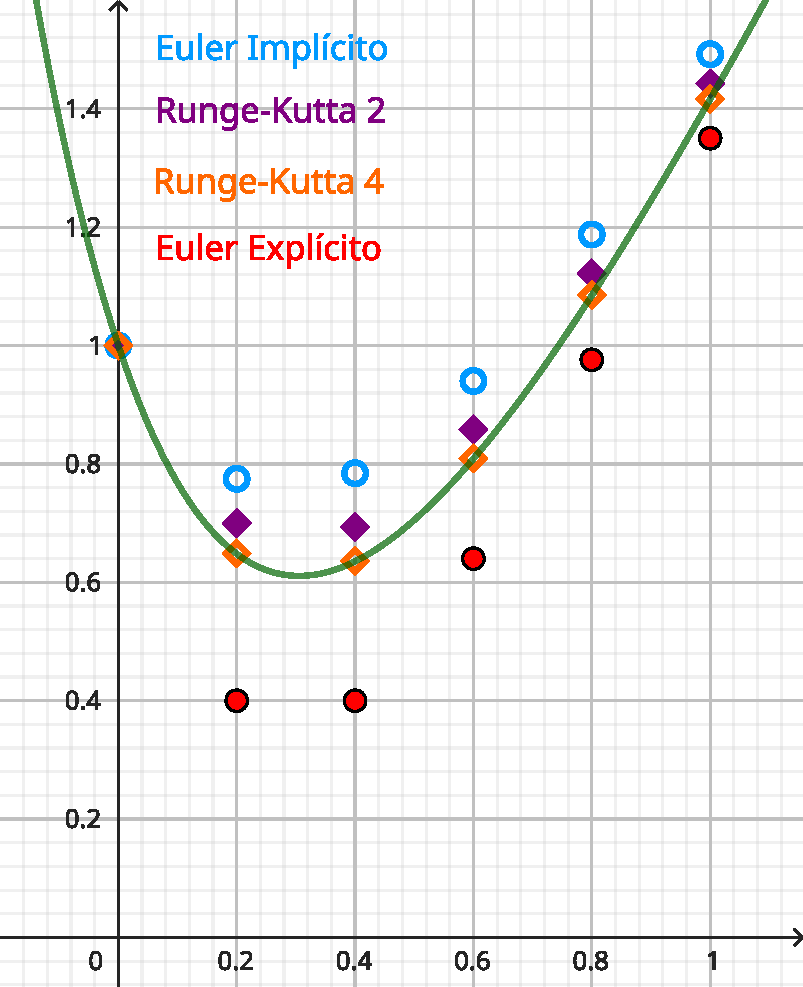
\includegraphics[width=0.4\textwidth]{img/22-equações-diferenciais-comparação.pdf}
\end{center}
\end{enumerate}
\end{document}
